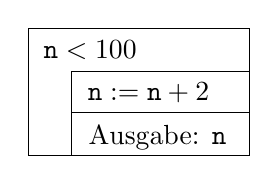
\begin{tikzpicture}
    \draw (0pt,0pt) rectangle (80.0pt, -46.1456pt);
    \node at (4.0pt, -23.0728pt) {};
    \node at (22.38681pt, -7.74239pt) {$\texttt{n} < 100$};
    \draw (15.48478pt,-15.48478pt) rectangle (80.0pt, -30.54144pt);
    \node at (43.4834pt, -23.46936pt) {$\texttt{n} := \texttt{n} + 2$};
    \draw (15.48478pt,-30.54144pt) rectangle (80.0pt, -46.1456pt);
    \node at (46.722895pt, -39.408105pt) {Ausgabe: $\texttt{n}$};
\end{tikzpicture}
